\documentclass[11pt, a4paper]{report}
\usepackage[utf8]{inputenc}
\usepackage{graphicx}
\usepackage{amsmath, amsfonts, amssymb}
\usepackage{mathtools}
\usepackage{tcolorbox}
\usepackage{fancyhdr}
\pagenumbering{arabic}
\usepackage{lipsum}
\usepackage{ulem}
\usepackage{geometry}
\parindent 0pt
\usepackage{float}
\usepackage{lscape}
\usepackage{siunitx}
\usepackage{xcolor}
\usepackage{listings}
\usepackage{multicol}
\usepackage[hidelinks]{hyperref}
\usepackage{bm}
\usepackage{subfigure}
\usepackage{subcaption}
\usepackage{booktabs}
\usepackage{tabularx}
\usepackage{comment}
\usepackage{soul}
\usepackage{fontspec}
\usepackage{minted2}
\usepackage{fancyvrb}
%\setmonofont{JetBrains Mono}

\setmonofont{Courier New}
\setmainfont{Arial}


\newfontfamily\codefont{Courier New}[Scale=1]

\renewcommand{\theFancyVerbLine}{%
    {\codefont\small\arabic{FancyVerbLine}}%
}

% \setminted{
%     linenos,
%     fontsize=\small
% }
\setminted{
  bgcolor=lightgray,
  breaklines=true,
  tabsize=4,
  linenos
}

%dependencies from mert 
\usepackage[capitalize]{cleveref}
\usepackage{color}
\usepackage{tcolorbox}


\definecolor{lightgray}{gray}{0.95}
\usepackage{witharrows} %for using the arrows inside math mode.

\usepackage{tikz}
\usetikzlibrary{arrows.meta,positioning,fit} 
\AtBeginEnvironment{minted}{
	\renewcommand{\itshape}{}}


\geometry{margin = 2cm}
% \pagestyle{fancy}
% \fancyhf{}
\renewcommand{\sectionmark}[1]{\markboth{#1}{}} % Remove section numbers
\renewcommand{\subsectionmark}[1]{\markright{#1}{}} % Remove subsection numbers
% \fancyhead[L]{\leftmark}
% \fancyfoot[C]{\thepage}
% \renewcommand{\headrulewidth}{0.3 pt}
% \renewcommand{\footrulewidth}{0.3 pt}

\begin{document}

\tableofcontents

\newpage

\chapter{SOC : $\sqrt[3]{y}$}
\section{calculation of the cube root}
\begin{figure}[!h]
\centering 
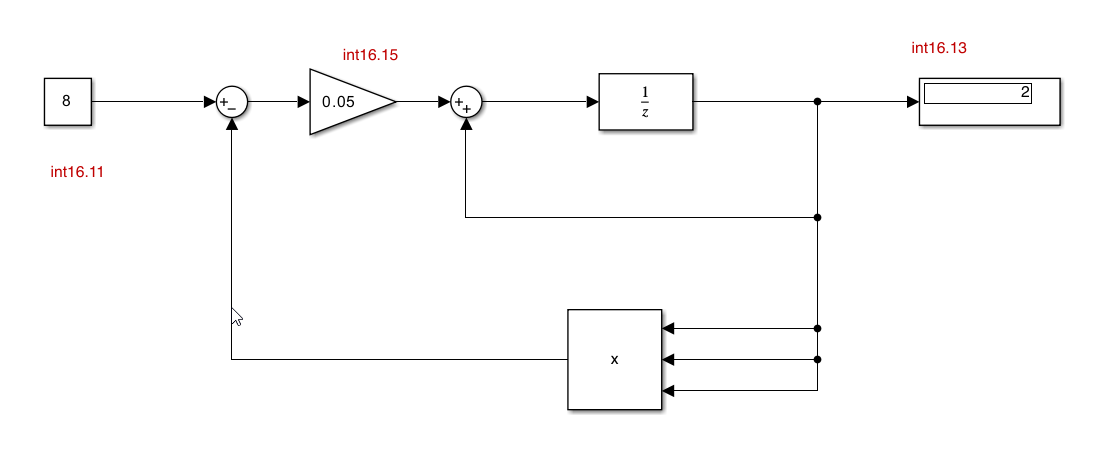
\includegraphics[width = 0.7\textwidth]{media/fig1.png}
\caption{The system to calculate the cube of the input}
\end{figure}
The following code is the implementation of the above algorithm in vhdl: 
\begin{minted}{vhdl}
----------------------------------------------------------------
-- Engineer: Mohammad Mahdi Mohammadi 
-- Create Date: 06/15/2026 11:07:11 AM
-- Module Name: cube - Behavioral
-- Description: accelerated cube root calcuation 
-- Revision: 2
-- Revision 0.01 - File Created
----------------------------------------------------------------
LIBRARY IEEE;
USE IEEE.STD_LOGIC_1164.ALL;
USE IEEE.NUMERIC_STD.ALL;

ENTITY cube IS
    PORT (
        clk, resetn, start : IN STD_LOGIC;
        done : OUT STD_LOGIC;
        u : IN STD_LOGIC_VECTOR(15 DOWNTO 0);
        y : OUT STD_LOGIC_VECTOR(15 DOWNTO 0));
END cube;

ARCHITECTURE Behavioral OF cube IS

    --signal and data formate declaration for y^3 fsm 
    TYPE r3_state_type IS (idle, st1, st2, st3, st4);
    SIGNAL r3_state : r3_state_type;

    SUBTYPE int16_t IS INTEGER RANGE -32768 TO 32767;
    SUBTYPE int32_t IS INTEGER RANGE -2147483648 TO 2147483647;

    SIGNAL r3_in : int16_t := 16384;
    SIGNAL r3_out : int16_t := 0;
    SIGNAL r3_temp : int32_t;
    SIGNAL r3_done : STD_LOGIC := '0';
    SIGNAL r3_start : STD_LOGIC := '1';

    --signal and datatype declaration for the main fsm 
    TYPE main_state_type IS (sidle, sst1, sst2, sst3, sst4, sst5, sst6);
    SIGNAL main_state : main_state_type;
    SIGNAL main_in, main_out : int16_t;
    SIGNAL main_temp : int32_t;

    SUBTYPE counter_type IS INTEGER RANGE 0 TO 25;
    CONSTANT iteration : INTEGER := 25;
    CONSTANT k01 : INTEGER := 1639; --k01 = 0.05 in int16.15
BEGIN

    --fsm y^3 
    fsm_r3_p : PROCESS (clk, resetn)
    BEGIN
        IF rising_edge(clk) THEN
            IF resetn = '0' THEN
                r3_state <= idle;
                r3_out <= 0;
            ELSE
                --default cases
                r3_done <= '0';
                CASE r3_state IS
                    WHEN idle =>
                        r3_done <= '1';
                        r3_temp <= 0;
                        IF r3_start = '1' THEN
                            r3_state <= st1;
                        END IF;
                    WHEN st1 =>
                        r3_temp <= r3_in * r3_in;
                        r3_state <= st2;
                    WHEN st2 =>
                        r3_temp <= (r3_temp)/2 ** 13;
                        r3_state <= st3;
                    WHEN st3 =>
                        r3_temp <= r3_temp * r3_in;
                        r3_state <= st4;
                    WHEN st4 =>
                        r3_out <= r3_temp / (2 ** 15);
                        r3_state <= idle;
                END CASE;
            END IF;
        END IF;
    END PROCESS fsm_r3_p;
    --fsm root cube calcuation 
    fsm_root_cube : PROCESS (clk, resetn)
        VARIABLE cnt : counter_type := 0;
    BEGIN
        IF rising_edge(clk) THEN
            IF resetn = '0' THEN
                main_state <= sidle;
                main_temp <= 0;
                main_out <= 0;
                cnt := 0;
            ELSE
                --default cases 
                done <= '0';
                CASE main_state IS
                    WHEN sidle =>
                        done <= '1';
                        cnt := 0;
                        main_temp <= 0;
                        main_in <= to_integer(signed(u));
                        main_out <= 8192; --initializing the y(k) to 1.0 in int16.13  
                        IF start = '1' THEN
                            main_state <= sst1;
                        END IF;
                    WHEN sst1 =>
                        IF cnt = iteration THEN
                            main_state <= sst6;
                        ELSE
                            --calculating the y^3 
                            r3_in <= main_out;
                            r3_start <= '1';
                            main_state <= sst2;
                        END IF;
                    WHEN sst2 =>
                        r3_start <= '0';
                        IF r3_done = '1' THEN
                            main_temp <= (main_in - r3_out); --int16.11 
                            main_state <= sst3;
                        END IF;
                    WHEN sst3 =>
                        main_temp <= k01 * main_temp;
                        main_state <= sst4;
                    WHEN sst4 =>
                        main_temp <= main_temp / (2 ** 13);
                        main_state <= sst5;
                    WHEN sst5 =>
                        main_out <= main_out + main_temp;
                        cnt := cnt + 1;
                        main_state <= sst1;
                    WHEN sst6 =>
                        y <= STD_LOGIC_VECTOR(to_signed(main_out, y'length));
                        main_state <= sidle;
                END CASE;
            END IF;
        END IF;
    END PROCESS fsm_root_cube;
END Behavioral;
\end{minted}
The following code shows the testbench for the above systems. 
\begin{minted}{vhdl}
--------------------------------------------------------
-- Engineer: Mohammad Mahdi Mohammadi 
-- Create Date: 06/15/2026 11:07:11 AM
-- Module Name: cube - Behavioral
-- Description: accelerated cube root calcuation 
-- Revision: 2
-- Revision 0.01 - File Created
--------------------------------------------------------
LIBRARY IEEE;
USE IEEE.STD_LOGIC_1164.ALL;
USE IEEE.NUMERIC_STD.ALL;
ENTITY cube_tb IS
END cube_tb;

ARCHITECTURE Behavioral OF cube_tb IS
    COMPONENT cube IS
        PORT (
            clk, resetn, start : IN STD_LOGIC;
            done : OUT STD_LOGIC;
            u : IN STD_LOGIC_VECTOR(15 DOWNTO 0);
            y : OUT STD_LOGIC_VECTOR(15 DOWNTO 0));
    END COMPONENT cube;
    SIGNAL clk, start, done : STD_LOGIC := '0';
    SIGNAL resetn : STD_LOGIC := '1';
    SIGNAL u : STD_LOGIC_VECTOR(15 DOWNTO 0) := x"0000";
    SIGNAL y : STD_LOGIC_VECTOR(15 DOWNTO 0) := x"0000";

    CONSTANT clk_period : TIME := 10 ns;

BEGIN

    --clock generation 
    clk <= NOT clk AFTER clk_period/2;

    --unit under test 
    uut : cube
    PORT MAP(
        clk => clk,
        resetn => resetn,
        start => start,
        done => done,
        u => u,
        y => y);

    --stimulus process 
    stim_p : PROCESS
    BEGIN
        start <= '1';
        resetn <= '1';
        u <= STD_LOGIC_VECTOR(to_signed(16384, 16));
        WAIT FOR clk_period * 40;

        WAIT;
    END PROCESS stim_p;

END Behavioral;
\end{minted}

\begin{figure}[!h]
\centering 
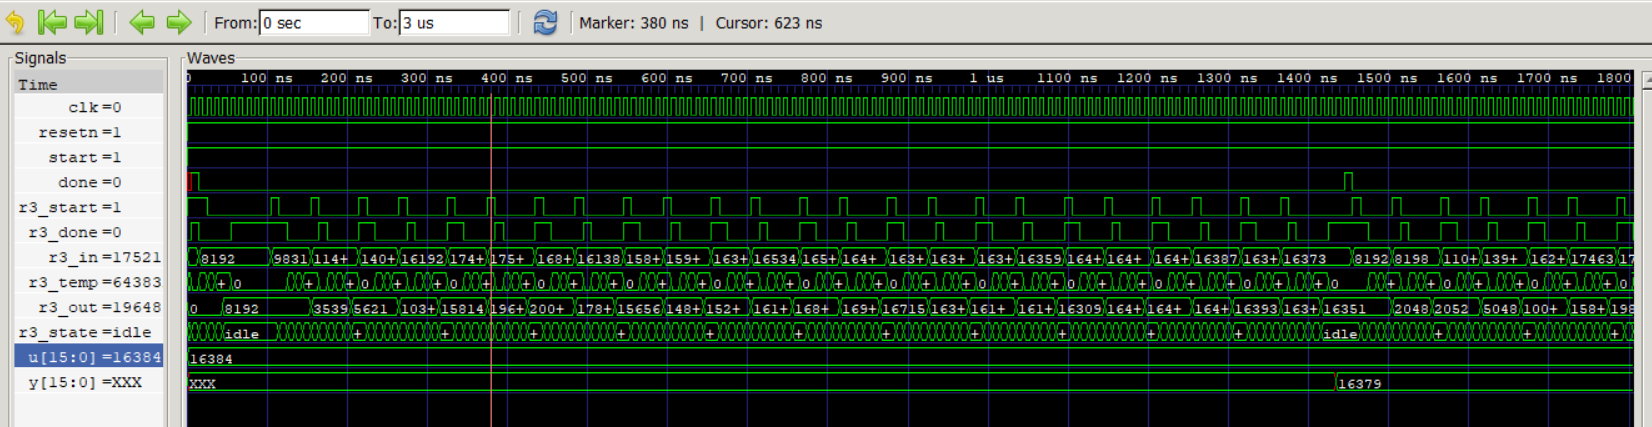
\includegraphics[width = 1\textwidth]{media/fig2.png}
\caption{The system simulation using GHDL}
\end{figure}

\section{C application code}
The following code shows the c application built for this system. 
\begin{minted}{c}
/*
 * helloworld.c: simple test application
 *
 * This application configures UART 16550 to baud rate 9600.
 * PS7 UART (Zynq) is not initialized by this application, since
 * bootrom/bsp configures it to baud rate 115200
 *
 * ------------------------------------------------
 * | UART TYPE   BAUD RATE                        |
 * ------------------------------------------------
 *   uartns550   9600
 *   uartlite    Configurable only in HW design
 *   ps7_uart    115200 (configured by bootrom/bsp)
 */

#include <stdio.h>
#include "platform.h"
#include "xil_printf.h"
#include <string.h>
#include <unistd.h>

#include "xparameters.h"

#define reg(k) *(volatile unsigned int*)(XPAR_CUBE_ROOT_0_S00_AXI_BASEADDR + 4*k)
#define cmd_len 128
#define nreg 4

void print_help(){
	printf("x      : to exit the program \n");
	printf("h      : to show this help menur \n");
	printf("start  : to start the calculation algorithm \n");
	printf("test   : to test the peripherals \n");
}

void my_getline(char *cmd, int size){
	int i = 0;
	char c;
	for(i = 0; i < size - 1; i++){
		c = getchar();
		if(c == '\r' || c == '\n'){
			c = '\0';
			putchar('\n');
			putchar('\r');
			break;
		}
		cmd[i] = c;
		putchar(c);
	}
	cmd[i] = '\0';
}

int main()
{
	int terminat = 0;
	char cmd[cmd_len];
	int xdata;

    init_platform();
    print_help();
    do{
    	printf(">> "); fflush(stdout);
    	my_getline(cmd, cmd_len);
    	if(!strcmp(cmd, "x")){
    		terminat = 1;
    	} else if(!strcmp(cmd, "h")){
    		print_help();
    	} else if(!strcmp(cmd, "start")){
    		printf("enter the value to find the 3rd root \n");
    		my_getline(cmd, cmd_len);
    		double data0;
    		sscanf(cmd, "%lf", &data0);
    		if(data0 <= 0 || data0 > 10){
    		    printf("value out of range, please enter a value between 0 and 10\n\r");
    		    continue;  // go back to prompt, not break
    		}
    		xdata = (int)(data0 *(1 << 11));
    		reg(1) = xdata & 0xffff;

    		//triggering the start signal
    		reg(2) = 1;

    		//poling untill done is high
    		do{
    			xdata = reg(2);
    			usleep(10);
    		}while(!(xdata & 0x1));
    		short int y_raw = (short int)(reg(1) & 0xffff);  // sign-extend correctly
    		double data = (double)y_raw / (double)(1 << 13);

    		printf("the 3rd root of %lf is %lf \n", data0, data);
    	} else if(!strcmp(cmd, "test")){
    		printf("1. leds \n");
    		printf("2. push buttons \n");
    		printf("3. switches \n");

    		int choice;
    		printf("select one of the above options  \n");
    		my_getline(cmd, cmd_len);
    		sscanf(cmd, "%d", &choice);

    		switch (choice) {
    		case 1:
    			printf("enter the value to be written to the leds \n");
    			my_getline(cmd, cmd_len);
    			sscanf(cmd, "%d", &xdata);
    			reg(0) = xdata;
    			break;

    		case 2:
    			printf("the push buttons will be read \n");
    			xdata = reg(0);
    			int pushbutton = (xdata >> 2) & 0xf;
    			printf("the value of the push buttons are : %x \n", pushbutton);
    			break;

    		case 3:
    			printf("the push buttons will be read \n");
				xdata = reg(0);
				int sw = (xdata) & 0x3;
				printf("the value of the switches are : %x \n", sw);
				break;

    		default:
    			printf("you did not enter a valid input \n");
    			break;

    		}

    	}
    }while(terminat == 0);
    print("Hello World\n\r");
    print("Successfully ran Hello World application");
    cleanup_platform();
    return 0;
}
\end{minted}

\newpage
\section{ Better Method, $\sqrt[3]{y}$}
The following code shows the implementation for the calculation of the cube root using one FSM method. 

\subsection{Source code file for cube root}
The following code shows the source code implementation of the cube root calcuation. 

\begin{minted}{vhdl}
LIBRARY ieee;
USE ieee.std_logic_1164.ALL;
USE ieee.numeric_std.ALL;

ENTITY s25 IS
    PORT (
        clk : IN STD_LOGIC;
        reset : IN STD_LOGIC;
        start : IN STD_LOGIC;
        done : OUT STD_LOGIC;
        x_in : IN STD_LOGIC_VECTOR(15 DOWNTO 0);
        y : OUT STD_LOGIC_VECTOR(15 DOWNTO 0)
    );
END ENTITY s25;

ARCHITECTURE behavioral OF s25 IS
    TYPE state_type IS (idle, init, state_cube0, state_cube1, state_cube2, state_root0, state_root1);
    SIGNAL state, next_state : state_type;

    SUBTYPE int16_t IS INTEGER RANGE -32768 TO 32767;
    SUBTYPE int32_t IS INTEGER RANGE -2147483648 TO 2147483647;
    SUBTYPE counter_type IS INTEGER RANGE 0 TO 25;

    CONSTANT input_frac : INTEGER := 11;
    CONSTANT output_frac : INTEGER := 13;
    CONSTANT iteration : INTEGER := 25;
    CONSTANT k0 : INTEGER := 1639; -- 0.05 in (int16_15)

    SIGNAL yk, yk1 : int16_t;
    SIGNAL temp, temp_i : int32_t;

    SIGNAL counter, counter_i : counter_type;
BEGIN

    -- sequential process 
    seq_p : PROCESS (clk)
    BEGIN
        IF rising_edge(clk) THEN
            IF reset = '1' THEN
                state <= idle;
                yk <= 0;
                temp <= 0;
                counter <= 0;
            ELSE
                state <= next_state;
                yk <= yk1;
                counter <= counter_i;
                temp <= temp_i;
            END IF;
        END IF;
    END PROCESS;

    -- combinational process
    comb_p : PROCESS (state, counter, start, yk, temp, x_in)
    BEGIN
        --default cases 
        next_state <= state;
        done <= '0';
        yk1 <= yk;
        counter_i <= counter;
        temp_i <= temp;

        CASE state IS
            WHEN idle =>
                done <= '1';
                IF start = '1' THEN
                    next_state <= init;
                END IF;
            WHEN init =>
                yk1 <= 0;
                counter_i <= 0;
                temp_i <= 0;
                next_state <= state_cube0;
            WHEN state_cube0 =>
                temp_i <= yk * yk;
                next_state <= state_cube1;
            WHEN state_cube1 =>
                temp_i <= (temp / (2 ** 13)) * yk;
                next_state <= state_cube2;
            WHEN state_cube2 =>
                temp_i <= temp / (2 ** 15);
                next_state <= state_root0;
            WHEN state_root0 =>
                temp_i <= (to_integer(signed(x_in)) - temp) * k0;
                next_state <= state_root1;
            WHEN state_root1 =>
                yk1 <= yk + temp/(2 ** 13);
                IF counter < iteration THEN
                    counter_i <= counter + 1;
                END IF;

                IF counter = iteration THEN
                    next_state <= idle;
                ELSE
                    next_state <= state_cube0;
                END IF;
        END CASE;
    END PROCESS;

    y <= STD_LOGIC_VECTOR(to_signed(yk, y'length));

END ARCHITECTURE behavioral;
\end{minted}

\subsection{Testbench code for the calculation of cube root}
The following code shows the testbench for the above implementation.

\begin{minted}{vhdl}
LIBRARY ieee;
USE ieee.std_logic_1164.ALL;
USE ieee.numeric_std.ALL;

ENTITY s25_tb IS
END ENTITY;

ARCHITECTURE behavioral OF s25_tb IS
    COMPONENT s25 IS
        PORT (
            clk : IN STD_LOGIC;
            reset : IN STD_LOGIC;
            start : IN STD_LOGIC;
            done : OUT STD_LOGIC;
            x_in : IN STD_LOGIC_VECTOR(15 DOWNTO 0);
            y : OUT STD_LOGIC_VECTOR(15 DOWNTO 0)
        );
    END COMPONENT s25;
    SIGNAL clk : STD_LOGIC := '0';
    SIGNAL reset, start, done : STD_LOGIC;
    SIGNAL x_in : STD_LOGIC_VECTOR(15 DOWNTO 0);
    SIGNAL y : STD_LOGIC_VECTOR(15 DOWNTO 0);

    CONSTANT clk_period : TIME := 10 ns;
BEGIN

    -- clock generation 
    clk <= NOT clk AFTER clk_period/2;

    -- unit under test 
    uut : s25
    PORT MAP(
        clk => clk,
        reset => reset,
        start => start,
        done => done,
        x_in => x_in,
        y => y
    );

    -- stimulus process 
    stim_p : PROCESS
    BEGIN
        start <= '1';
        reset <= '0';
        x_in <= STD_LOGIC_VECTOR(to_signed(16384, x_in'length));
        WAIT FOR clk_period;
        start <= '0';
        WAIT FOR clk_period * 100;
        WAIT;
    END PROCESS;

END ARCHITECTURE behavioral;
\end{minted}

The following figure shows the simulation result of the above implementation using GHDL. \\ 
it shows the input value of 16384 which is equal to 8.0 in \texttt{int16\_11} format and the output value of 8192 which is equal to 2.0 in \texttt{int16\_13} format.

\begin{figure}[H]
	\centering
	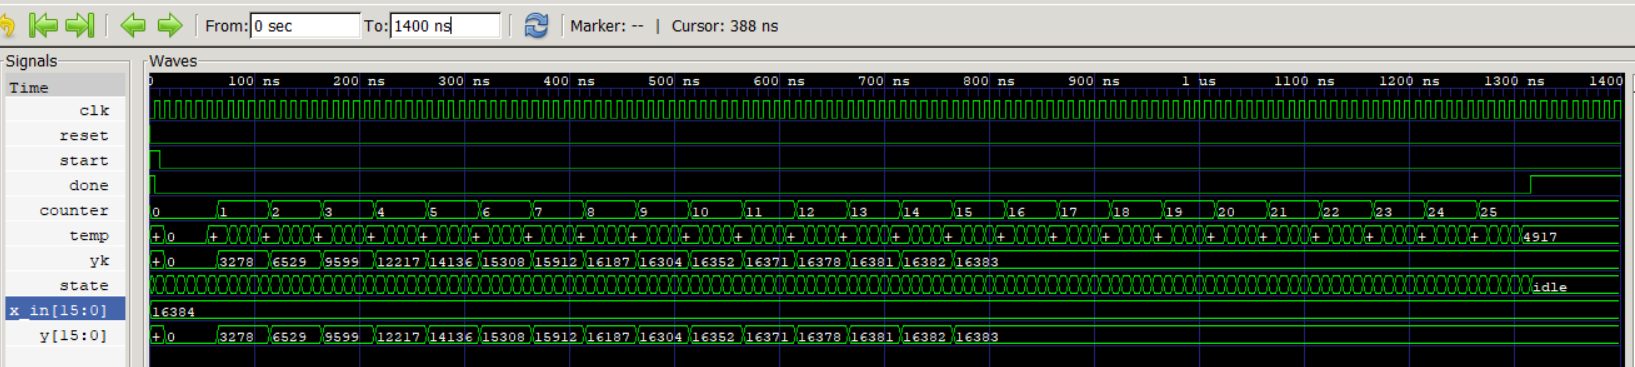
\includegraphics[width = 1\textwidth]{media/y3source.png}
	\caption{Simulation result of the cube root implementation}
\end{figure}



\newpage
\section{Zerocrossing}
\begin{figure}[!h]
\centering 
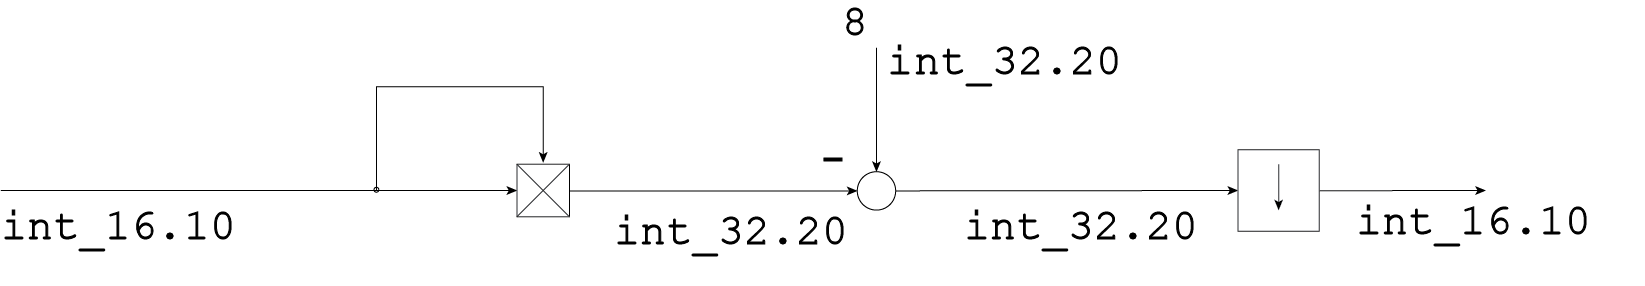
\includegraphics[width = 0.8\textwidth]{media/s24.png}
\caption{function calculation figure}
\end{figure}

The following vhdl code is the solution. 
\begin{minted}{vhdl}
LIBRARY ieee;
USE ieee.std_logic_1164.ALL;
USE ieee.numeric_std.ALL;

ENTITY zerocross IS
    PORT (
        clk, resetn, start : IN STD_LOGIC;
        done               : OUT STD_LOGIC;
        rightv, leftv      : IN  STD_LOGIC_VECTOR(15 DOWNTO 0);
        newx, newy         : OUT STD_LOGIC_VECTOR(15 DOWNTO 0)
    );
END zerocross;

ARCHITECTURE behavioral OF zerocross IS

    TYPE fcalc_state_type IS (idle, st1, st2, st3);
    SIGNAL fcalc_state : fcalc_state_type := idle;

    SUBTYPE int16_t IS INTEGER RANGE -32768 TO 32767;
    SUBTYPE int32_t IS INTEGER RANGE -2147483648 TO 2147483647;

    SIGNAL fcalc_xin   : int16_t := 0;
    SIGNAL fcalc_yout  : int16_t := 0;
    SIGNAL fcalc_temp  : int32_t := 0;
    SIGNAL fcalc_done  : STD_LOGIC := '0';
    SIGNAL fcalc_start : STD_LOGIC := '0';

    TYPE main_state_type IS (sidle, init, sst1, sst1b, sst2, sst3, sst4, final);
    SIGNAL main_state : main_state_type := sidle;

    SUBTYPE counter_type IS INTEGER RANGE 0 TO 30;
    SIGNAL count : counter_type := 0;

    SIGNAL rightv_i, leftv_i : int16_t := 0;
    SIGNAL newx_i, newy_i    : int16_t := 0;
    CONSTANT iteration        : INTEGER := 15;

BEGIN

    -- function FSM: f(x) = 8 - x^2
    f_calc_process : PROCESS (clk)
    BEGIN
        IF rising_edge(clk) THEN
            IF resetn = '0' THEN
                fcalc_state <= idle;
                fcalc_temp  <= 0;
                fcalc_yout  <= 0;
                fcalc_done  <= '0';
            ELSE
                fcalc_done <= '0';  -- default

                CASE fcalc_state IS
                    WHEN idle =>
                        -- no fcalc_done here
                        IF fcalc_start = '1' THEN
                            fcalc_state <= st1;
                        END IF;

                    WHEN st1 =>
                        fcalc_temp  <= fcalc_xin * fcalc_xin;  -- Q20
                        fcalc_state <= st2;

                    WHEN st2 =>
                        fcalc_temp  <= 8388608 - fcalc_temp;   -- 8.0 in Q20
                        fcalc_state <= st3;

                    WHEN st3 =>
                        fcalc_yout  <= fcalc_temp / (2**10);   -- Q20 -> Q10
                        fcalc_done  <= '1';                    -- only here
                        fcalc_state <= idle;

                END CASE;
            END IF;
        END IF;
    END PROCESS f_calc_process;

    -- bisection main FSM
    zerocross_p : PROCESS (clk)
        VARIABLE cnt : counter_type := 0;
    BEGIN
        IF rising_edge(clk) THEN
            IF resetn = '0' THEN
                main_state <= sidle;
                newx_i     <= 0;
                newy_i     <= 0;
                rightv_i   <= 0;
                leftv_i    <= 0;
                count      <= 0;
                cnt        := 0;
            ELSE
                done        <= '0';  -- default
                fcalc_start <= '0';  -- default

                CASE main_state IS

                    WHEN sidle =>
                        done <= '1';
                        IF start = '1' THEN
                            cnt        := 0;
                            count      <= 0;
                            main_state <= init;
                        END IF;

                    WHEN init =>
                        rightv_i   <= to_integer(signed(rightv));
                        leftv_i    <= to_integer(signed(leftv));
                        main_state <= sst1;

                    WHEN sst1 =>
                        IF cnt = iteration THEN
                            main_state <= final;
                        ELSE
                            -- compute midpoint, wait one cycle for signal to settle
                            newx_i     <= (rightv_i + leftv_i) / 2;
                            main_state <= sst1b;
                        END IF;

                    WHEN sst1b =>
                        -- newx_i is now valid, feed to function block
                        fcalc_xin   <= newx_i;
                        fcalc_start <= '1';
                        main_state  <= sst2;

                    WHEN sst2 =>
                        -- wait for function FSM to complete
                        IF fcalc_done = '1' THEN
                            -- fcalc_yout valid on next cycle
                            main_state <= sst3;
                        END IF;

                    WHEN sst3 =>
                        -- fcalc_yout is now stable
                        newy_i     <= fcalc_yout;
                        main_state <= sst4;

                    WHEN sst4 =>
                        IF newy_i < 0 THEN
                            rightv_i <= newx_i;
                        ELSE
                            leftv_i  <= newx_i;
                        END IF;
                        cnt        := cnt + 1;
                        count      <= cnt;
                        main_state <= sst1;

                    WHEN final =>
                        newx       <= STD_LOGIC_VECTOR(to_signed(newx_i, newx'length));
                        newy       <= STD_LOGIC_VECTOR(to_signed(newy_i, newy'length));
                        done       <= '1';
                        main_state <= sidle;

                END CASE;
            END IF;
        END IF;
    END PROCESS zerocross_p;

END ARCHITECTURE behavioral;
\end{minted}

\section{Testbench file}
The following code is the testbench file of the above porgram
\begin{minted}{vhdl}
LIBRARY ieee;
USE ieee.std_logic_1164.ALL;
USE ieee.numeric_std.ALL;

ENTITY zerocross_tb IS
END zerocross_tb;

ARCHITECTURE behavioral OF zerocross_tb IS
	COMPONENT zerocross IS
		PORT (
			clk, resetn, start : IN STD_LOGIC;
			done : OUT STD_LOGIC;
			rightv, leftv : IN STD_LOGIC_VECTOR(15 DOWNTO 0);
			newx, newy : OUT STD_LOGIC_VECTOR(15 DOWNTO 0)
		);
	END COMPONENT zerocross;
	SIGNAL clk, start : STD_LOGIC := '0';
	SIGNAL resetn : STD_LOGIC := '1';
	SIGNAL done : STD_LOGIC;
	SIGNAL rightv, leftv : STD_LOGIC_VECTOR(15 DOWNTO 0) := (OTHERS => '0');
	SIGNAL newx, newy : STD_LOGIC_VECTOR(15 DOWNTO 0) := (OTHERS => '0');

	--signals for the clock generation 
	CONSTANT clk_period : TIME := 10 ns;

BEGIN
	--clock generation 
	clk <= NOT clk AFTER clk_period/2;

	--unit under test 
	uut : zerocross
	PORT MAP(
		clk => clk,
		resetn => resetn,
		start => start,
		done => done,
		rightv => rightv,
		leftv => leftv,
		newx => newx,
		newy => newy
	);

	--stimulus process 
	stim_p : PROCESS
	BEGIN
		rightv <= STD_LOGIC_VECTOR(to_signed(4096, 16));
		leftv <= STD_LOGIC_VECTOR(to_signed(-4096, 16));
		
		-- reset pulse
		resetn <= '0';
		WAIT FOR clk_period * 2;
		resetn <= '1';
		WAIT FOR clk_period;
		
		start <= '1'; 
		resetn <= '1'; 
		wait for clk_period; 
		start <= '0';
		WAIT FOR clk_period * 200;
		
		
		WAIT;
	END PROCESS stim_p;
END behavioral;
\end{minted}

\begin{figure}[!h]
\centering 
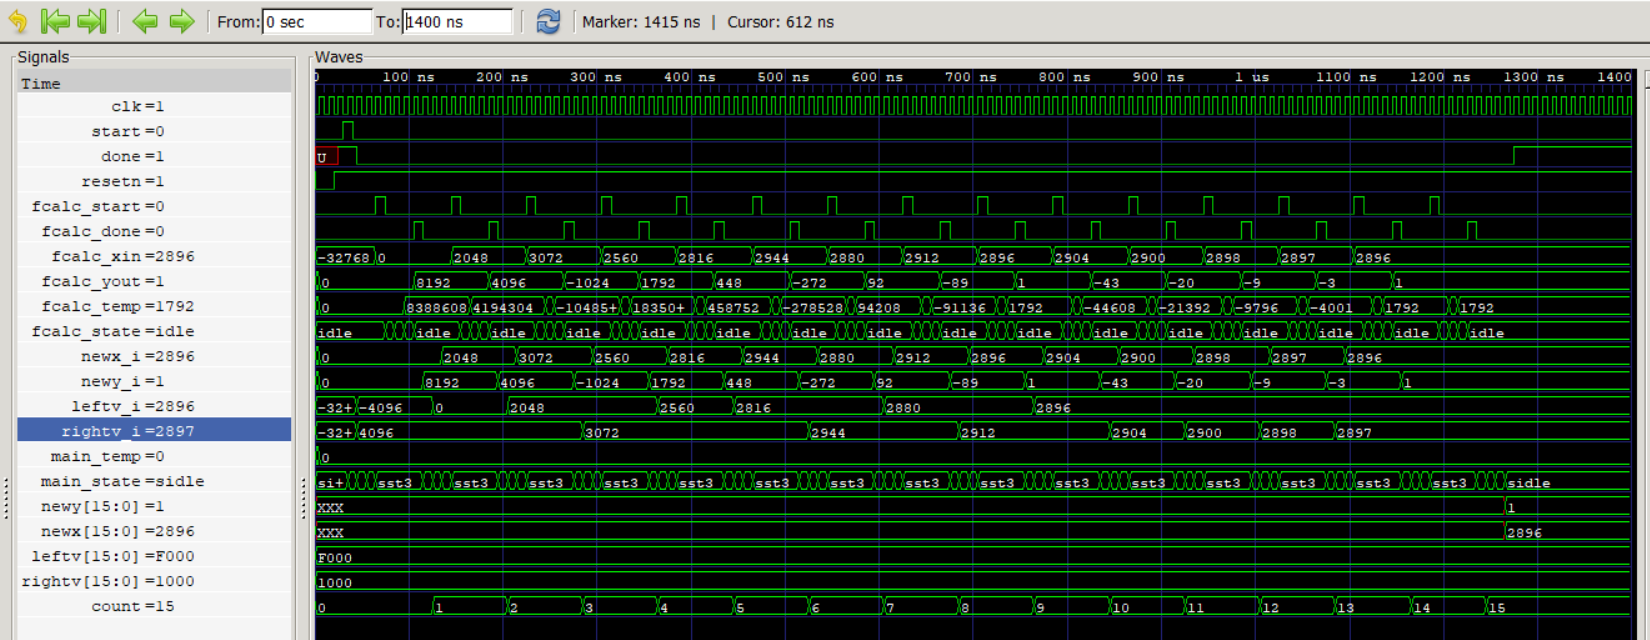
\includegraphics[width = 1\textwidth]{media/s24b.png}
\caption{output of zerocrossing detector}
\end{figure}

\section{IP generation}
The following code shows the vhdl code for reading and writing the registers. 
\begin{minted}{vhdl}
-- Implement memory mapped register select and write logic generation
	-- The write data is accepted and written to memory mapped registers when
	-- axi_awready, S_AXI_WVALID, axi_wready and S_AXI_WVALID are asserted. Write strobes are used to
	-- select byte enables of slave registers while writing.
	-- These registers are cleared when reset (active low) is applied.
	-- Slave register write enable is asserted when valid address and data are available
	-- and the slave is ready to accept the write address and write data.
	slv_reg_wren <= axi_wready and S_AXI_WVALID and axi_awready and S_AXI_AWVALID ;

	process (S_AXI_ACLK)
	variable loc_addr :std_logic_vector(OPT_MEM_ADDR_BITS downto 0);
	begin
	  if rising_edge(S_AXI_ACLK) then
	    if S_AXI_ARESETN = '0' then
	      slv_reg0 <= (others => '0');
	      slv_reg1 <= (others => '0');
	      slv_reg2 <= (others => '0');
	      slv_reg3 <= (others => '0');
		  start <= '0';
	    else
		  start <= '0';
	      loc_addr := axi_awaddr(ADDR_LSB + OPT_MEM_ADDR_BITS downto ADDR_LSB);
	      if (slv_reg_wren = '1') then
	        case loc_addr is
	          when b"00" =>
	            for byte_index in 0 to (C_S_AXI_DATA_WIDTH/8-1) loop
	              if ( S_AXI_WSTRB(byte_index) = '1' ) then
	                -- Respective byte enables are asserted as per write strobes
	                -- slave registor 0
	                slv_reg0(byte_index*8+7 downto byte_index*8) <= S_AXI_WDATA(byte_index*8+7 downto byte_index*8);
	              end if;
	            end loop;
	          when b"01" =>
	            for byte_index in 0 to (C_S_AXI_DATA_WIDTH/8-1) loop
	              if ( S_AXI_WSTRB(byte_index) = '1' ) then
	                -- Respective byte enables are asserted as per write strobes
	                -- slave registor 1
	                slv_reg1(byte_index*8+7 downto byte_index*8) <= S_AXI_WDATA(byte_index*8+7 downto byte_index*8);
	              end if;
	            end loop;
	          when b"10" =>
				start <= '1';
	            for byte_index in 0 to (C_S_AXI_DATA_WIDTH/8-1) loop
	              if ( S_AXI_WSTRB(byte_index) = '1' ) then
	                -- Respective byte enables are asserted as per write strobes
	                -- slave registor 2
	                slv_reg2(byte_index*8+7 downto byte_index*8) <= S_AXI_WDATA(byte_index*8+7 downto byte_index*8);
	              end if;
	            end loop;
	          when b"11" =>
	            for byte_index in 0 to (C_S_AXI_DATA_WIDTH/8-1) loop
	              if ( S_AXI_WSTRB(byte_index) = '1' ) then
	                -- Respective byte enables are asserted as per write strobes
	                -- slave registor 3
	                slv_reg3(byte_index*8+7 downto byte_index*8) <= S_AXI_WDATA(byte_index*8+7 downto byte_index*8);
	              end if;
	            end loop;
	          when others =>
	            slv_reg0 <= slv_reg0;
	            slv_reg1 <= slv_reg1;
	            slv_reg2 <= slv_reg2;
	            slv_reg3 <= slv_reg3;
	        end case;
	      end if;
	    end if;
	  end if;
	end process;
	
	
	-- Implement memory mapped register select and read logic generation
		-- Slave register read enable is asserted when valid address is available
		-- and the slave is ready to accept the read address.
		slv_reg_rden <= axi_arready and S_AXI_ARVALID and (not axi_rvalid) ;
	
		process (leftv, rightv, newx, done, newy, axi_araddr, S_AXI_ARESETN, slv_reg_rden)
		variable loc_addr :std_logic_vector(OPT_MEM_ADDR_BITS downto 0);
		begin
		    -- Address decoding for reading registers
		    loc_addr := axi_araddr(ADDR_LSB + OPT_MEM_ADDR_BITS downto ADDR_LSB);
		    case loc_addr is
		      when b"00" =>
		        reg_data_out <= x"0000" & leftv;
		      when b"01" =>
		        reg_data_out <= x"0000" & rightv;
		      when b"10" =>
		        reg_data_out <= x"000" & "000" & newx & done;
		      when b"11" =>
		        reg_data_out <= x"0000" & newy;
		      when others =>
		        reg_data_out  <= (others => '0');
		    end case;
		end process;
		
		leftv <= slv_reg0(15 downto 0);
  		rightv <= slv_reg1(15 downto 0);
\end{minted}

The following code shows the c application for the above program 
\begin{minted}{c}
/*
 * helloworld.c: simple test application
 *
 * This application configures UART 16550 to baud rate 9600.
 * PS7 UART (Zynq) is not initialized by this application, since
 * bootrom/bsp configures it to baud rate 115200
 *
 * ------------------------------------------------
 * | UART TYPE   BAUD RATE                        |
 * ------------------------------------------------
 *   uartns550   9600
 *   uartlite    Configurable only in HW design
 *   ps7_uart    115200 (configured by bootrom/bsp)
 */

#include <stdio.h>
#include "platform.h"
#include "xil_printf.h"
#include <string.h>
#include <unistd.h>

#include "xparameters.h"

#define reg(k) *(volatile unsigned int *)(XPAR_ZCROSS_0_S00_AXI_BASEADDR + (4*k))
#define cmd_len 64

void print_help(){
	printf("h     : to show this help menu \n");
	printf("x     : to close the application \n");
	printf("start : to start the calculation \n");
}

void my_getline(char *cmd, int size){
	int i;
	char c;
	for(i = 0; i < size - 1; i++){
		c = getchar();
		if(c == '\r' || c == '\n'){
			c = '\0';
			putchar('\r');
			putchar('\n');
			break;
		}
		cmd[i] = c;
		putchar(c);
	}
	cmd[i] = '\0';
}

int main()
{
	int terminat = 0;
	char cmd[cmd_len];
	unsigned int xdata;
    init_platform();

    print_help();
    do{
    	printf(">> "); fflush(stdout);
    	my_getline(cmd, cmd_len);
    	if(!strcmp(cmd, "x")){
    		terminat = 1;
    	} else if(!strncmp(cmd, "write", 5)){
    		unsigned int regnum;
    		unsigned int regval;
    		if(sscanf(cmd, "write %d %d", &regnum, &regval) != 2){
    			printf("the value was wrote correctly, right usage is write <regnum> <regval> \n");
    		} else {
    			reg(regnum) = regval;
    			printf("the value %d has been written to reg%d. \n", regval, regnum);
    		}
    	} else if(!strcmp(cmd, "start")){
    		double rightv_f, leftv_f;
    		unsigned int rightv, leftv;
    		printf("please enter the value for rightv and leftv. (int_16.10), <rightv> <leftv> \n");
    		my_getline(cmd, cmd_len);
    		if(sscanf(cmd, "%lf %lf", &rightv_f, &leftv_f) != 2){
    			printf("you did not enter the values correctly \n");
    		} else {
    			rightv = (unsigned int)(rightv_f * (1 << 10));
    			leftv = (unsigned int)(leftv_f * (1 << 10));

    			reg(0) = leftv;
    			reg(1) = rightv;
    			printf("%d : has be written to reg(0) \n", leftv);
    			printf("%d : has be written to reg(1) \n", rightv);

    			//triggering the start signal
    			reg(2) = 1;

    			//polling for done signal
    			do{
    				xdata = reg(2);
    				usleep(10);
    			}while(!(xdata & 0x1));
    			printf("done flage raised \n");

    			//xdata = reg(2);
    			printf("xdata = reg(2) = %d \n", xdata);

    			short unsigned int newx, newy;
    			double newx_f, newy_f;
    			xdata = (xdata >> 1);
    			newx = *(short unsigned int*)&(xdata);
    			newx_f = (double)newx / (double)(1 << 10);

    			xdata = reg(3);
    			printf("xdata = %d \n", xdata);
    			newy = *(short unsigned int*)&(xdata);
    			newy_f = (double)newy / (double)(1 << 10);

    			printf("the zerocrossing value for this program has been found \n");
    			printf("the zerocrossing is : %d (%lf) \n", newx, newx_f);
    			printf("the correspoding y value is : %d (%lf) \n", newy, newy_f);
    		}
    	}
    }while(terminat == 0);

    print("Thanks for using the zcross application\n\r");
    print("Successfully ran application");
    cleanup_platform();
    return 0;
}
\end{minted}

\newpage
\section{Zerocrossing calculation (Better Method, Single FSM)}
The zerocrossing method has been implemented using a single FSM method. The following code shows the implementation of the zerocrossing calculation using a single FSM method.

\subsection{Source Code}
The following code shows the source code for the zerocrossing calculation using a single FSM method.
\begin{minted}{vhdl}
LIBRARY ieee;
USE ieee.std_logic_1164.ALL;
USE ieee.numeric_std.ALL;

ENTITY s24 IS
    PORT (
        clk : IN STD_LOGIC;
        reset : IN STD_LOGIC;
        start : IN STD_LOGIC;
        done : OUT STD_LOGIC;
        xin : IN STD_LOGIC_VECTOR(31 DOWNTO 0);
        yout : OUT STD_LOGIC_VECTOR(15 DOWNTO 0)
    );
END ENTITY s24;

ARCHITECTURE behavioral OF s24 IS
    TYPE state_type IS (idle, init, state1, state2, state3, state4, state5);
    SIGNAL state, next_state : state_type;
    SUBTYPE int16_t IS INTEGER RANGE -32768 TO 32767;
    SUBTYPE int32_t IS INTEGER RANGE -2147483648 TO 2147483647;
    SUBTYPE counter_type IS INTEGER RANGE 0 TO 15;

    CONSTANT rightv_init : int16_t := 4096; -- 4 in int16_10 
    CONSTANT leftv_init : int16_t := 1024; -- 1 in int16_10 

    SIGNAL counter, counter_i : counter_type;
    SIGNAL temp, temp_i : int32_t;
    SIGNAL newx : int16_t := 0;
    SIGNAL leftv, leftv_i, rightv, rightv_i : int16_t;

BEGIN

    -- sequential process 
    seq_p : PROCESS (clk)
    BEGIN
        IF rising_edge(clk) THEN
            IF reset = '1' THEN
                state <= idle;
                counter <= 0;
                temp <= 0;
                rightv <= 0;
                leftv <= 0;
            ELSE
                state <= next_state;
                counter <= counter_i;
                temp <= temp_i;
                leftv <= leftv_i;
                rightv <= rightv_i;
            END IF;
        END IF;
    END PROCESS seq_p;

    -- combinational process 
    comb_p : PROCESS (state, start, counter)
    BEGIN
        -- default cases 
        done <= '0';
        next_state <= state;
        counter_i <= counter;
        temp_i <= temp;
        leftv_i <= leftv;
        rightv_i <= rightv;

        CASE state IS
            WHEN idle =>
                done <= '1';
                IF start = '1' THEN
                    next_state <= init;
                END IF;
            WHEN init =>
                rightv_i <= rightv_init;
                leftv_i <= leftv_init;
                counter_i <= 0;
                newx <= 0;
                next_state <= state1;
            WHEN state1 =>
                newx <= (leftv + rightv)/2;
                next_state <= state2;
            WHEN state2 =>
                temp_i <= (newx * newx);
                next_state <= state3;
            WHEN state3 =>
                temp_i <= (temp - to_integer(signed(xin)));
                next_state <= state4;
            WHEN state4 =>
                temp_i <= temp / (2 ** 13);
                IF counter <= 15 THEN
                    counter_i <= counter + 1;
                END IF;
                next_state <= state5;
            WHEN state5 =>
                IF temp >= 0 THEN
                    rightv_i <= newx;
                ELSE
                    leftv_i <= newx;
                END IF;
                IF counter = 15 THEN
                    next_state <= idle;
                ELSE
                    next_state <= state1;
                END IF;
        END CASE;
    END PROCESS comb_p;

    yout <= STD_LOGIC_VECTOR(to_signed(newx, yout'length));

END ARCHITECTURE behavioral;
\end{minted}

\subsection{Zerocrossing algorithm Testbench file}
The following code shows the testbench for the above implementation of the zerocrossing calculation using a single FSM method.

\begin{minted}{vhdl}
LIBRARY ieee;
USE ieee.std_logic_1164.ALL;
USE ieee.numeric_std.ALL;

ENTITY s24_tb IS
END ENTITY;

ARCHITECTURE behavioral OF s24_tb IS
    COMPONENT s24 IS
        PORT (
            clk : IN STD_LOGIC;
            reset : IN STD_LOGIC;
            start : IN STD_LOGIC;
            done : OUT STD_LOGIC;
            xin : IN STD_LOGIC_VECTOR(31 DOWNTO 0);
            yout : OUT STD_LOGIC_VECTOR(15 DOWNTO 0)
        );
    END COMPONENT;
    SIGNAL clk : STD_LOGIC := '0';
    SIGNAL reset, start, done : STD_LOGIC;
    SIGNAL xin : STD_LOGIC_VECTOR(31 DOWNTO 0);
    SIGNAL yout : STD_LOGIC_VECTOR(15 DOWNTO 0);

    CONSTANT clk_period : TIME := 10 ns;

BEGIN

    -- clock generation 
    clk <= NOT clk AFTER clk_period/2;

    -- unit under test 
    uut : s24
    PORT MAP(
        clk => clk,
        reset => reset,
        start => start,
        done => done,
        xin => xin,
        yout => yout
    );

    -- stimulus process 
    stim_p : PROCESS
    BEGIN
        reset <= '0';
        start <= '1';
        xin <= STD_LOGIC_VECTOR(to_signed(8388608, xin'length));
        WAIT FOR clk_period;
        start <= '0';
        WAIT FOR clk_period * 50;

        WAIT;
    END PROCESS;

END ARCHITECTURE behavioral;
\end{minted}

\subsection{Simulations Result}
The following figure shows the simulation result of the above implementation using GHDL. \\
It shows the input value of 8388608 which is equal to 8.0 in \texttt{int16\_10} format and the output value of 2894 which is equal to 2.8262 in \texttt{int16\_10} format.

\begin{figure}[H]
	\centering 
	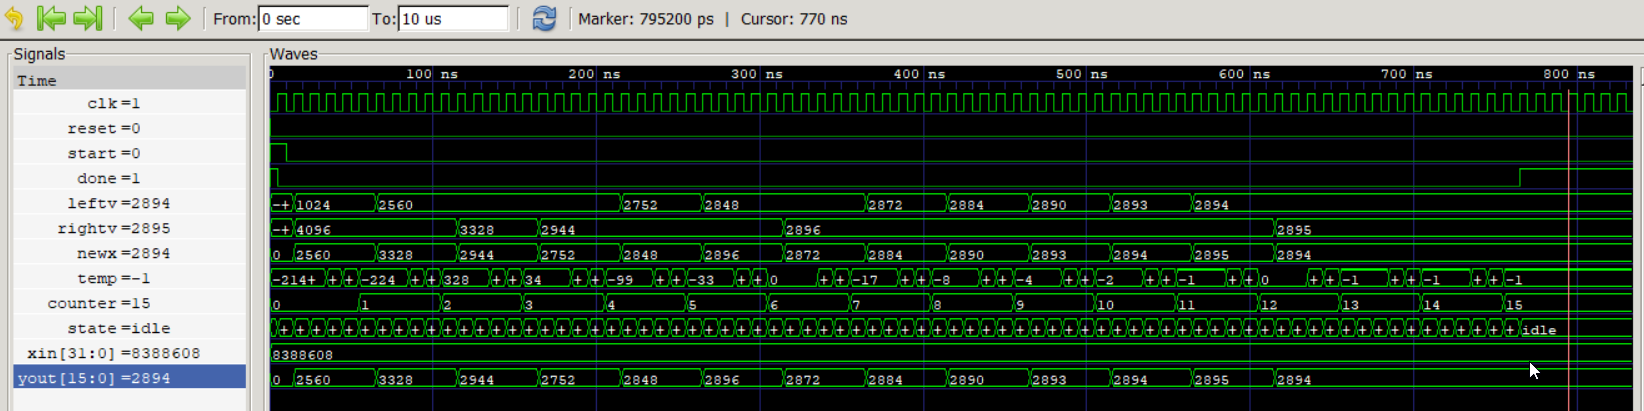
\includegraphics[width = 1\textwidth]{media/zcross_sim.png}
	\caption{Simulation result of the zerocrossing implementation}
\end{figure}
\end{document}




















